\documentclass[14pt, a4paper]{extreport}
\usepackage{extsizes}
\usepackage[a4paper, left=30mm, right=15mm, top=20mm, bottom=20mm]{geometry}
\usepackage[english, russian]{babel}
\usepackage{fontspec}
\defaultfontfeatures{Ligatures={TeX},Renderer=Basic}
\setmainfont[Ligatures={TeX,Historic}]{Times New Roman}
\usepackage{amsmath,amssymb}
\usepackage{graphicx}
\usepackage{setspace}
\graphicspath{{images/}}
\usepackage[hidelinks]{hyperref}
\usepackage{indentfirst}
\setlength{\parindent}{1.25cm}
\usepackage[explicit,compact]{titlesec}
\usepackage{titletoc}
\newcommand{\doublerule}[1][.4pt]{%
	\noindent
	\makebox[0pt][l]{\rule[.6ex]{\linewidth}{#1}}%
	\rule[.3ex]{\linewidth}{#1}
}

\addto\captionsrussian{%
	\renewcommand{\contentsname}%
	{\centering{СОДЕРЖАНИЕ}}%
}

\usepackage{caption}
\DeclareCaptionLabelSeparator{dash}{ -- }
\DeclareCaptionLabelFormat{figure}{Рисунок #2}
\captionsetup[table]{
	labelsep=dash,
	singlelinecheck=false,
}
\captionsetup[figure]{
	labelsep=dash,
	labelformat=figure,
}

\usepackage{floatrow}
\floatsetup[table]{style=plaintop}
\floatsetup[equation]{style=plain}

\usepackage{chngcntr}
\counterwithout{figure}{chapter}
\counterwithout{equation}{chapter}
\counterwithout{table}{chapter}

\usepackage{cleveref}
\crefformat{table}{смотри табл.#2#1#3}
\Crefformat{table}{Смотри табл.#2#1#3}

\crefformat{figure}{рис.~#2#1#3}
\Crefformat{figure}{Рис.~#2#1#3}
\crefmultiformat{figure}{рис.~#2#1#3}{,~#2#1#3}{,~#2#1#3}{,~#2#1#3}
\crefrangeformat{figure}{рис.~#3#1#4--#5#2#6}

\crefformat{equation}{#1}
\crefmultiformat{equation}{~#2#1#3}{,~#2#1#3}{,~#2#1#3}{,~#2#1#3}
\crefrangeformat{equation}{~#3#1#4--#5#2#6}

\usepackage{array}
\setlength{\extrarowheight}{.5ex}

\begin{document}
\begin{titlepage}
	\begin{center}
		\vspace*{0.5mm}
		\setstretch{1.1}

		
\includegraphics[width=0.18\textwidth]{logo}\\
		\footnotesize
		МИНИСТЕРСТВО НАУКИ И ВЫСШЕГО ОБРАЗОВАНИЯ РОССИЙСКОЙ ФЕДЕРАЦИИ\\
		\small
		Федеральное государственное бюджетное образовательное учреждение высшего образования\\
		\textbf{«МИРЭА - Российский технологический университет»}
		\vspace{0.5cm}

		\large \textbf{РТУ МИРЭА} \normalsize

		\doublerule[1pt]\\
		\vspace{0.4cm}

		Институт искусственного интеллекта\\
		Кафедра общей информатики
		\vspace{1.5cm}

		\textbf{ОТЧЕТ}\\
		\textbf{ПО ПРАКТИЧЕСКОЙ РАБОТЕ № 8}\\
		\textbf{реализация заданной логической функции от четырех переменных на мультиплексорах 16-1, 8-1, 4-1, 2-1}\\
		\textbf{по дисциплине}\\
		«ИНФОРМАТИКА»
		\vspace{1.5cm}

		\small
		Выполнил студент группы ИМБО-01-22 \hfill Скирдин Никита Сергеевич
		\vspace{1cm}

		Принял \hfill Павлова Екатерина Сергеевна\\
		ассистент \hfill
		\vspace{1.5cm}

		\footnotesize
		\hspace{0.5cm} Практическая \hfill «\_\_»\_\_\_\_\_\_2022 г. \hfill Подпись студента\\
		\hspace{0.5cm} работа выполнена \hfill
		\vspace{0.5cm}

		\hspace{2cm} «Зачтено» \hfill «\_\_»\_\_\_\_\_\_2022 г. \hfill Подпись преподавателя
		\vfill

		\small
		Москва 2022
	\end{center}
	\thispagestyle{empty}
\end{titlepage}

\setstretch{1.5}
\setcounter{page}{2}

\titlecontents{chapter}[0em]
	{\vskip 0.5ex}%
	{\thecontentslabel \space \uppercase}% numbered sections formatting
	{}% unnumbered sections formatting
	{\hfill \thecontentspage}%

\titlecontents{section}[1.25cm]
	{\vskip 0.5ex}%
	{\thecontentslabel \space}
	{}
	{\hfill \thecontentspage}

\titleformat{\chapter}[block]
	{\bfseries\normalsize}{}{0pt}{\uppercase{#1}}

\titleformat{\section}[block]
	{\bfseries\normalsize}{}{0pt}{#1}

\titlespacing*{\chapter}{0pt}{-10.5mm}{0pt}

\tableofcontents

\titleformat{\chapter}[display]
	{\centering\bfseries\normalsize}{}{0pt}{\thechapter \space \uppercase{#1}}

\titleformat{\section}[block]
	{\hspace{\parindent}\bfseries\normalsize}{}{0pt}{\thesection \space #1}

\titlespacing*{\chapter}{0pt}{-19.5mm}{0pt}

\chapter{Постановка задачи}
Логическая функция от четырех переменных задана в 16-теричной векторной форме. Восстановить таблицу истинности. По таблице истинности реализовать в лабораторном комплексе логическую функцию на мультиплексорах следующими способами:

– используя один мультиплексор 16-1;

– используя один мультиплексор 8-1;

– используя минимальное количество мультиплексоров 4-1;

– используя минимальную комбинацию мультиплексоров 4-1 и 2-1.

Протестировать работу схем и убедиться в их правильности. Подготовить отчет о проделанной работе и защитить ее.

\section{Персональный вариант}
Логическая функция от четырех переменных, заданная в 16-теричной форме: F9AA$_{16}$

\chapter{Проектирование и реализация}
\section{Предварительная подготовка данных}
Преобразуем заданную логическую функцию в двоичную запись: 1111 1001 1010 1010$_2$ - получили столбец значений логической функции, который необходим для восстановления полной таблицы истинности (\cref{tab:function-values}).

\begin{table}[!htbp]
	\caption{Таблица истинности заданной функции}
	\label{tab:function-values}
	\begin{tabular}{|c|c|c|c|c|}
		\hline
		a & b & c & d & F \\
		\hline
		0 & 0 & 0 & 0 & 1 \\
		\hline
		0 & 0 & 0 & 1 & 1 \\
		\hline
		0 & 0 & 1 & 0 & 1 \\
		\hline
		0 & 0 & 1 & 1 & 1 \\
		\hline
		0 & 1 & 0 & 0 & 1 \\
		\hline
		0 & 1 & 0 & 1 & 0 \\
		\hline
		0 & 1 & 1 & 0 & 0 \\
		\hline
		0 & 1 & 1 & 1 & 1 \\
		\hline
		1 & 0 & 0 & 0 & 1 \\
		\hline
		1 & 0 & 0 & 1 & 0 \\
		\hline
		1 & 0 & 1 & 0 & 1 \\
		\hline
		1 & 0 & 1 & 1 & 0 \\
		\hline
		1 & 1 & 0 & 0 & 1 \\
		\hline
		1 & 1 & 0 & 1 & 0 \\
		\hline
		1 & 1 & 1 & 0 & 1 \\
		\hline
		1 & 1 & 1 & 1 & 0 \\
		\hline
	\end{tabular}
\end{table}

\section{Реализация функции на мультиплексоре 16-1}
Количество информационных входов мультиплексора соответствует количеству значений логической функции. Поэтому просто подадим значения функции на соответствующие входы. На адресные (выбирающие) входы мультиплексора подадим при помощи шины значения логических переменных. Несмотря на использование шины, следует помнить, что младшая переменная подается на младший адресный вход, а старшая – на старший.

Собранная и протестированная схема показана на \cref{fig:multiplexer-16-1}.

\begin{figure}[H]
	\caption{Тестирование схемы, реализующей логическую функцию на мультиплексоре 16-1}
	\label{fig:multiplexer-16-1}
	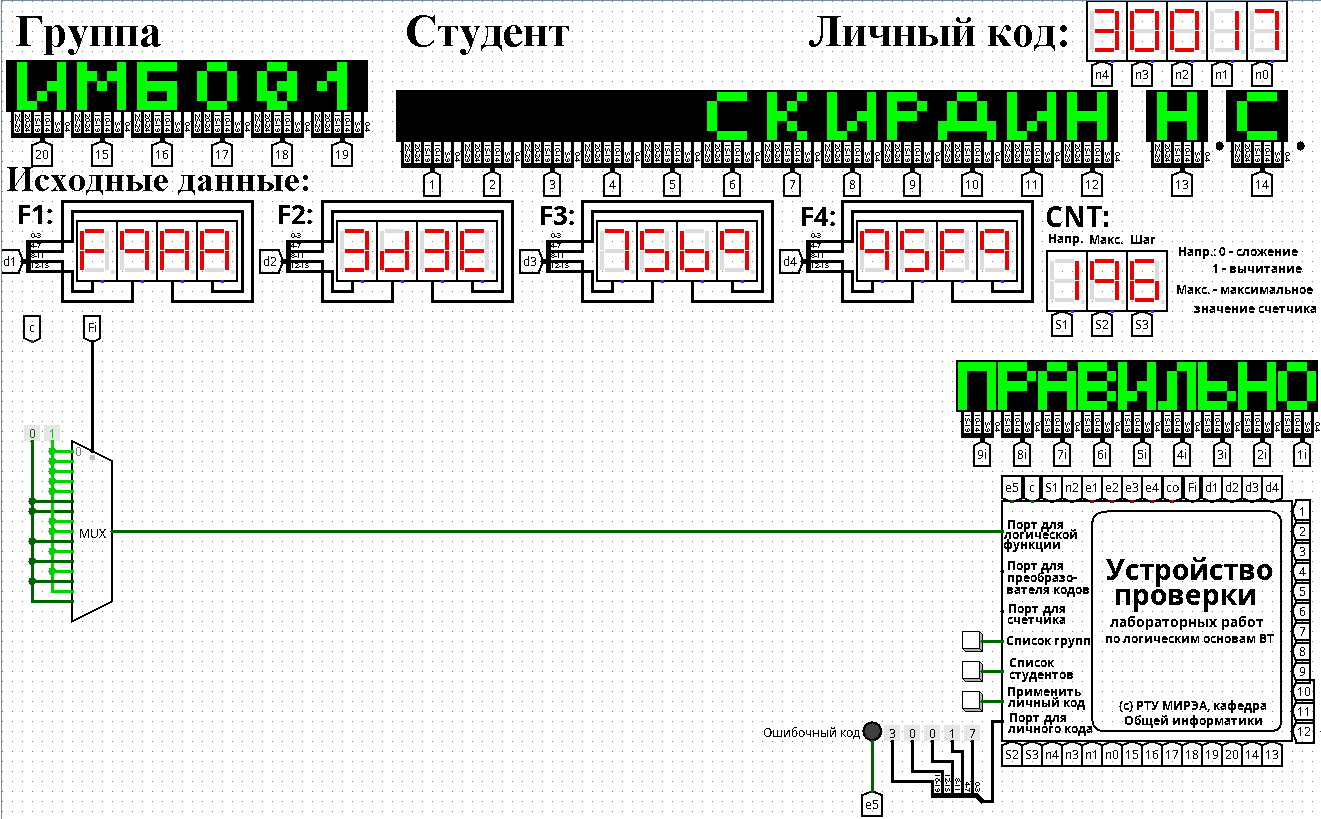
\includegraphics[width=\textwidth]{multiplexer-16-1}
\end{figure}

\section{Реализация функции на мультиплексоре 8-1}
Мультиплексор 8-1 имеет 3 адресных входа, что не позволяет подать на эти входы все 4 логические переменные.

Однако мы можем в качестве адресных переменных выбрать любые три из имеющихся, а оставшуюся четвертую рассматривать наравне с логическими константами как элемент исходных данных для информационных входов.

Удобнее всего в качестве адресных переменных взять три старшие переменные нашей функции, т.е. a, b, c. Тогда пары наборов, на которых эти переменные будут иметь одинаковое значение, будут располагаться в соседних строчках таблицы истинности и поэтому можно будет легко увидеть, как значение логической функции для каждой пары наборов соотносится со значением переменной d.

Таким образом, мы перенесли одну переменную в область значений функции и получили таблицу, похожую на таблицу истинности функции от трех переменных (\cref{tab:f-and-d-relation}).

\begin{table}[!htbp]
	\caption{Взаимосвязь значений функции и значений переменной d}
	\label{tab:f-and-d-relation}
	\begin{tabular}{|c|c|c|c|}
		\hline
		a & b & c & F \\
		\hline
		0 & 0 & 0 & 1 \\
		\hline
		0 & 0 & 1 & 1 \\
		\hline
		0 & 1 & 0 & $\overline{d}$ \\
		\hline
		0 & 1 & 1 & $d$ \\
		\hline
		1 & 0 & 0 & $\overline{d}$ \\
		\hline
		1 & 0 & 1 & $\overline{d}$ \\
		\hline
		1 & 1 & 0 & $\overline{d}$ \\
		\hline
		1 & 1 & 1 & $\overline{d}$ \\
		\hline
	\end{tabular}
\end{table}

Теперь, рассматривая переменную d наравне с константами 0 и 1 в качестве сигналов для информационных входов мультиплексора 8-1, можно по аналогии с предыдущим случаем выполнить реализацию требуемой функции.

Разместим на рабочей области новый мультиплексор, установим ему количество выбирающих (адресных) входов равным трем, и выполним необходимые соединения (\cref{fig:multiplexer-8-1}).

\begin{figure}[H]
	\caption{Тестирование схемы, реализующей логическую функцию на мультиплексоре 8-1}
	\label{fig:multiplexer-8-1}
	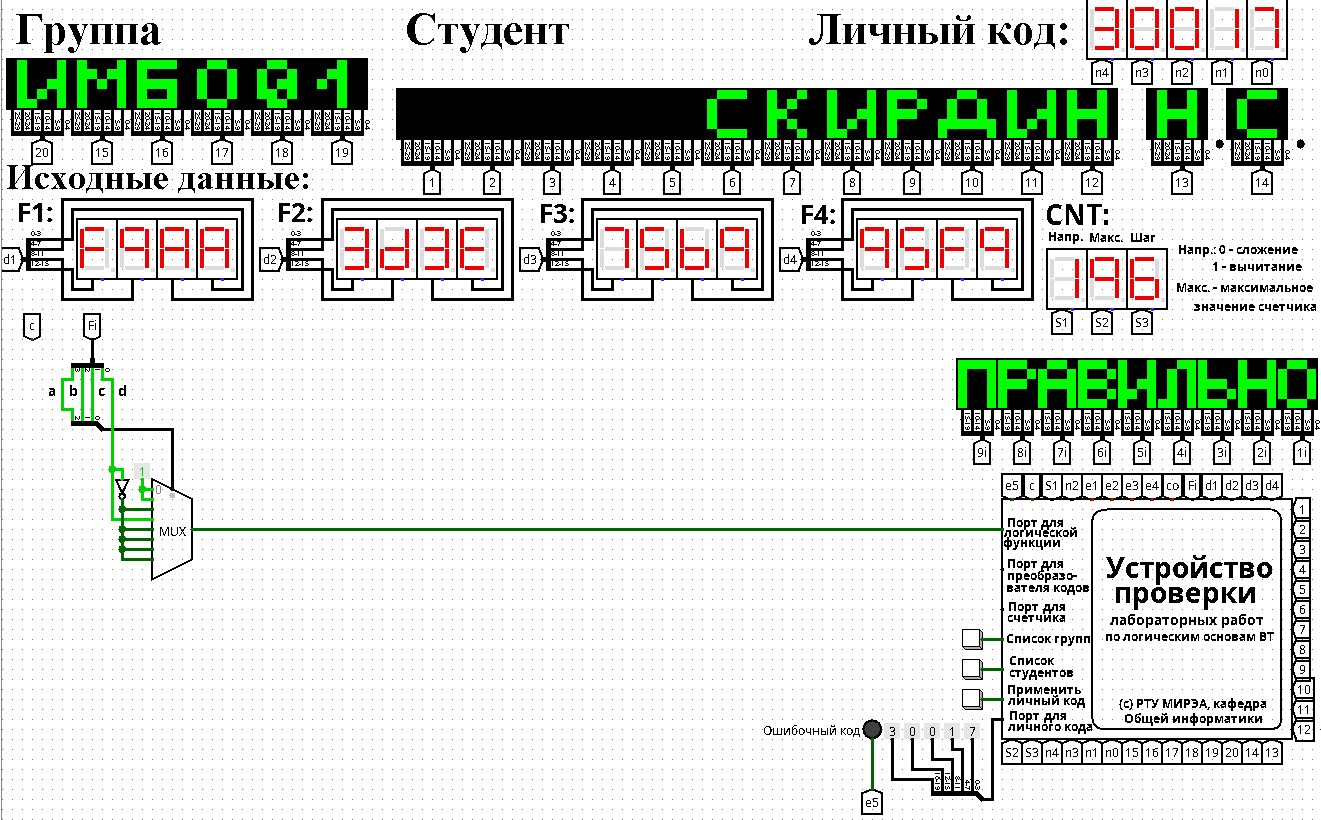
\includegraphics[width=\textwidth]{multiplexer-8-1}
\end{figure}

\section{Реализация функции на минимальном количестве мультиплексоров 4-1}
Мультиплексор 4-1 имеет 2 адресных входа и 4 информационных. Это означает, что мы должны разбить исходную таблицу истинности на 4 фрагмента, за реализацию каждого из которых в принципе должен отвечать отдельный мультиплексор (назовем его операционным). Однако, необходимо учесть требования минимальности по отношению к количеству используемых мультиплексоров и ставить их только там, где без них нельзя обойтись.

Для реализации схемы обязательно потребуется управляющий мультиплексор, который будет выбирать один из вариантов, предлагаемых операционными мультиплексорами (либо один из очевидных вариантов, если без операционных мультиплексоров можно обойтись).

В первой из четырех частей таблицы истинности (\cref{tab:function-values}) функция всегда принимает значение 1, во второй части понадобится мультиплексор, а в третьей и четвертой $F = \overline{d}$. Схема логической функции на минимальном количестве мультиплексоров 4-1 будет такой, как показано на \cref{fig:multiplexer-4-1}.

\begin{figure}[H]
	\caption{Тестирование схемы, реализующей логическую функцию на минимальном количестве мультиплексоров 4-1}
	\label{fig:multiplexer-4-1}
	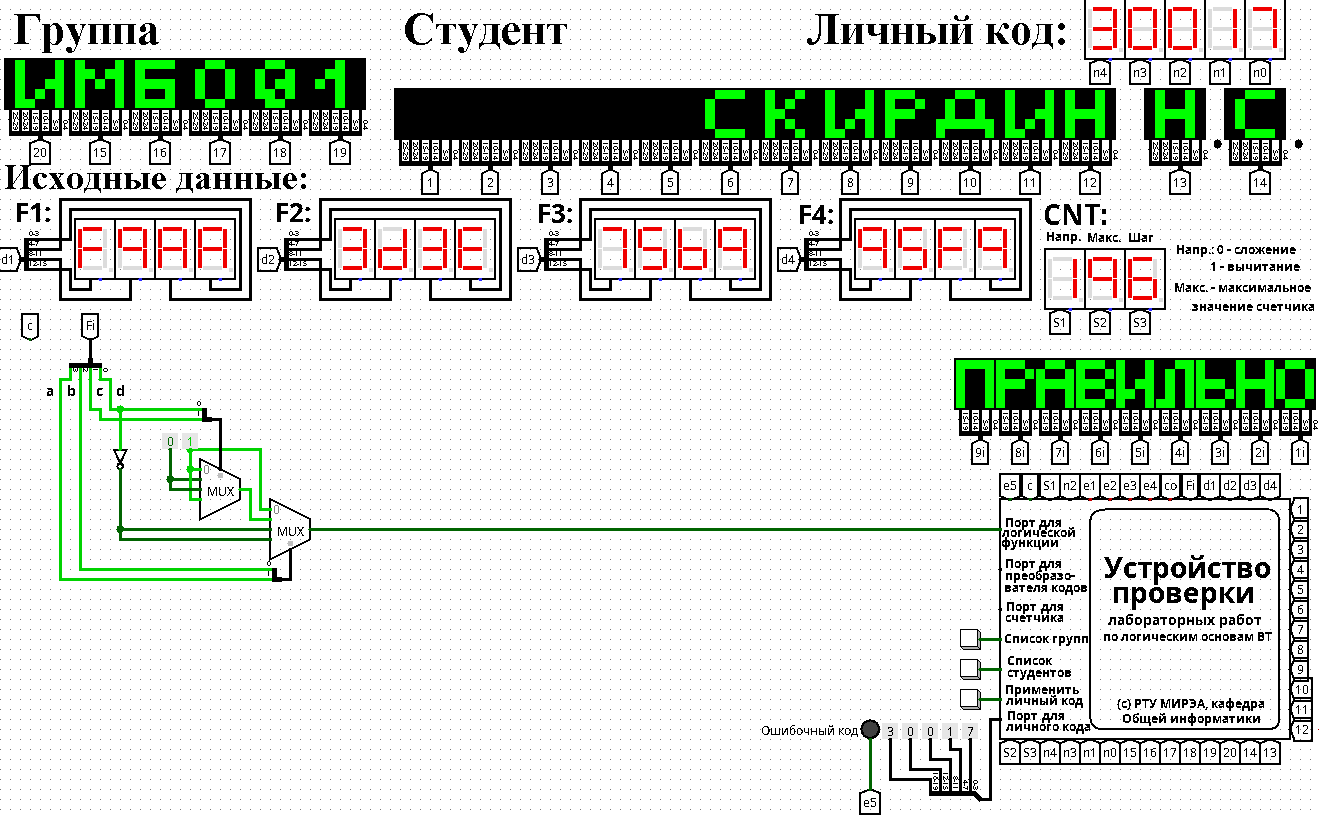
\includegraphics[width=\textwidth]{multiplexer-4-1}
\end{figure}

\section{Реализация функции на основе минимальной комбинации мультиплексоров 4-1 и 2-1}
Реализуем логическую функцию, используя минимальную комбинацию мультиплексоров 4-1 и 2-1. В качестве отправной точки рассмотрим результаты, полученные в предыдущей реализации. Управляющий мультиплексор нельзя заменить на мультиплексор 2-1, поскольку у него на входах уникальные сигналы, а вот единственный операционный заменить можно, поскольку он имеет дело с константами. Когда «с» равно 0, то $F = \overline{d}$, а когда «с» равно 1, то $F = d$. Значит, переменную «с» можно рассматривать как адресную для мультиплексора 2-1, а не «d» и «d» будут поданы на его информационные входы. В результате получим схему, изображенную на \cref{fig:multiplexer-2-1}.

\begin{figure}[H]
	\caption{Тестирование схемы, реализующей логическую функцию на основе минимальной комбинации мультиплексоров 4-1 и 2-1}
	\label{fig:multiplexer-2-1}
	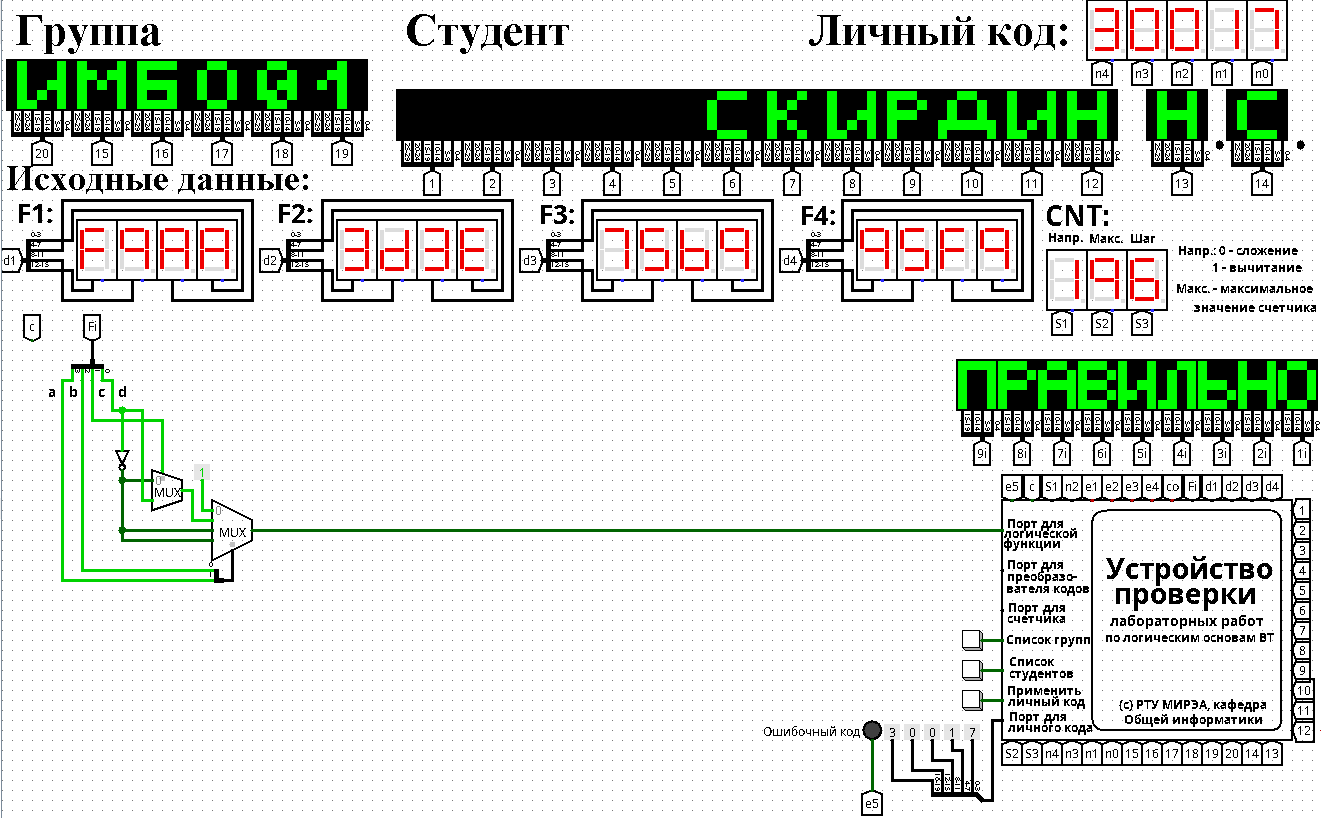
\includegraphics[width=\textwidth]{multiplexer-2-1}
\end{figure}

\chapter{Выводы}
В ходе работы была восстановлена таблица истинности логической функции от четырех переменных. По таблице истинности была реализована в лабораторном комплексе логическая функция на мультиплексорах следующими способами:

– используя один мультиплексор 16-1;

– используя один мультиплексор 8-1;

– используя минимальное количество мультиплексоров 4-1;

– используя минимальную комбинацию мультиплексоров 4-1 и 2-1.

Работа схем была протестирована, чтобы убедиться в правильности их работы.

\chapter{Информационный источник}
\textbf{Смирнов, С. С.} Информатика : Методические указания по выполнению практических работ / С. С. Смирнов, Д. А. Карпов. -- Москва : МИРЭА -- Российский технологический университет, 2020. -- 102 с.

\end{document}
